\section{How does pre-training time effect generalization performance?}
\label{sec:speed}
%Pre-Training is the process of initializing CNN parameters for a target application using images from a (generally larger) separate dataset. Features learned by a CNN pre-trained on Imagenet have been shown to generalize and achieve state of art results across multiple computer vision datasets (see section \ref{sec:fine} and \cite{Decaf}). Since, no single image dataset fully captures the variation in natural images, all datasets are biased (cite Alyosha). Consequently, it can be expected that excessive pre-training can cause the CNN to overfit on Imagenet and thus hurt generalization performance. 
There is no single image dataset which fully captures the variation in natural images. This means that all datasets including Imagenet are biased (cite Alyosha). Thus, there is a possibility that excessive pre-training can cause the CNN to overfit and consequently hurt generalization performance. Therefore, it is critical to address this issue and we investigated the effect of pre-training time on generalization performance with and without fine-tuning. We find that pre-training more improves performance. This is surprising, as it implies that fitting more to ImageNet leads to better performance when moving to other datasets. %The other interesting thing we note is that within 50K iterations of pre-training, the performance is almost 90\% of the final performance achieved after nearly 300K iterations.

\setlength{\tabcolsep}{4pt}
\begin{table}[t!]
\begin{center}
\caption{Performance variation (mAP) on PASCAL-CLS as a function of pre-training iterations on Imagenet.}
\label{table:det-traj-classify}
\begin{tabular}{lcccccccccc}
\hline\noalign{\smallskip}
Layer  & 5K & 15K & 25K & 35K & 50K & 95K & 105K & 195K & 205K & 305K \\
\noalign{\smallskip}
\hline
\noalign{\smallskip}
conv-1 & 23.0 & 24.3 & 24.4 & 24.5 & 24.3 & 24.8 & 24.7 & 24.4 & $24.4 \pm 0.5$ & -\\
conv-2 & 33.7 & 40.4 & 40.9 & 41.8 & 42.7 & 43.2 & 44.0 & 45.0 & $45.1 \pm 0.7$ & -\\
conv-3 & 34.2 & 46.8 & 47.0 & 48.2 & 48.6 & 49.4 & 51.6 & 50.7 & $50.9 \pm 0.6$ & -\\
conv-4 & 33.5 & 49.0 & 48.7 & 50.2 & 50.7 & 51.6 & 54.1 & 54.3 & $54.4 \pm 0.6$ & -\\
conv-5 & 33.0 & 53.4 & 55.0 & 56.8 & 57.3 & 59.2 & 63.5 & 64.9 & $65.5 \pm 0.3$ & -\\
fc-6   & 34.2 & 59.7 & 62.6 & 62.7 & 63.5 & 65.6 & 69.3 & 71.3 & $71.8 \pm 0.3$ & -\\
fc-7   & 30.9 & 61.3 & 64.1 & 65.1 & 65.9 & 67.8 & 71.8 & 73.4 & $74.0 \pm 0.3$ & -\\
\hline
\end{tabular}
\end{center}
\end{table}
\setlength{\tabcolsep}{1.4pt}

\setlength{\tabcolsep}{1pt}
\begin{table}[t!]
\begin{center}
\caption{Performance variation on SUN-CLS and PASCAL-DET using features from a CNN pre-trained for different number of iterations and fine-tuned for a fixed number of iterations (40K for SUN-CLS and 70K for PASCAL-DET)}
\label{table:det-trajectory}
\scalebox{1.00}{
\begin{tabular}{l|c|c|c|c}
 & 50K & 105K & 205K & 305K \\
\hline
\textbf{SUN-CLS} & 52.8 & 54.7 & 56.4 & 56.6 \\
\textbf{PASCAL-DET} & 50.2 & 52.6 & 55.3 & 55.4 \footnote{This number is different than 54.1 reported in \ref{sec:fine} probably due to difference in pre-training runs.}  \\
\end{tabular}}
\end{center}
\end{table}
\setlength{\tabcolsep}{1.4pt}

\begin{figure}[t!]
\centering
\subfloat[5K Iterations]{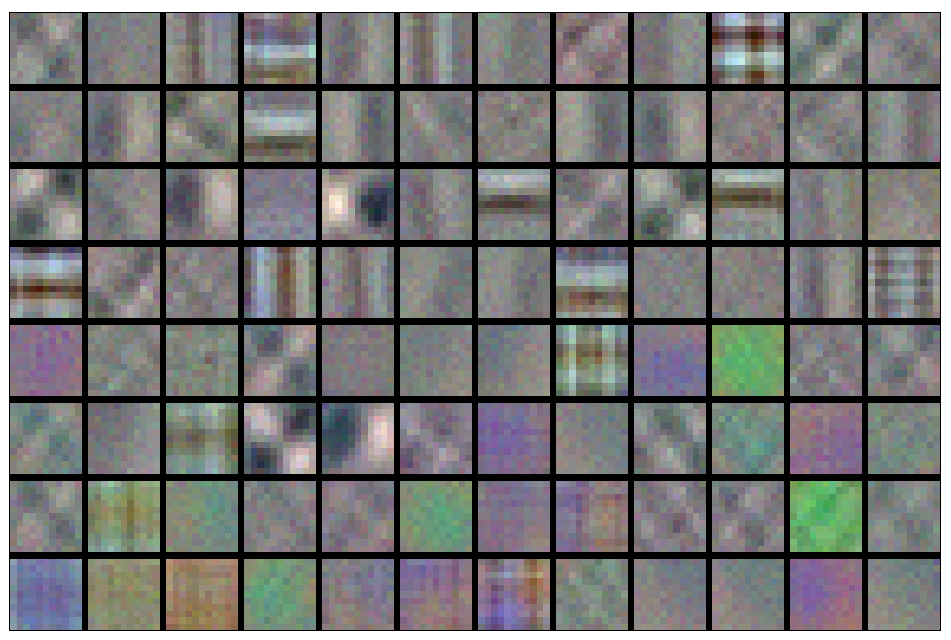
\includegraphics[scale=0.10]{images/l1_filters_iter5000.png}} \hspace{2mm}
\subfloat[15K Iterations]{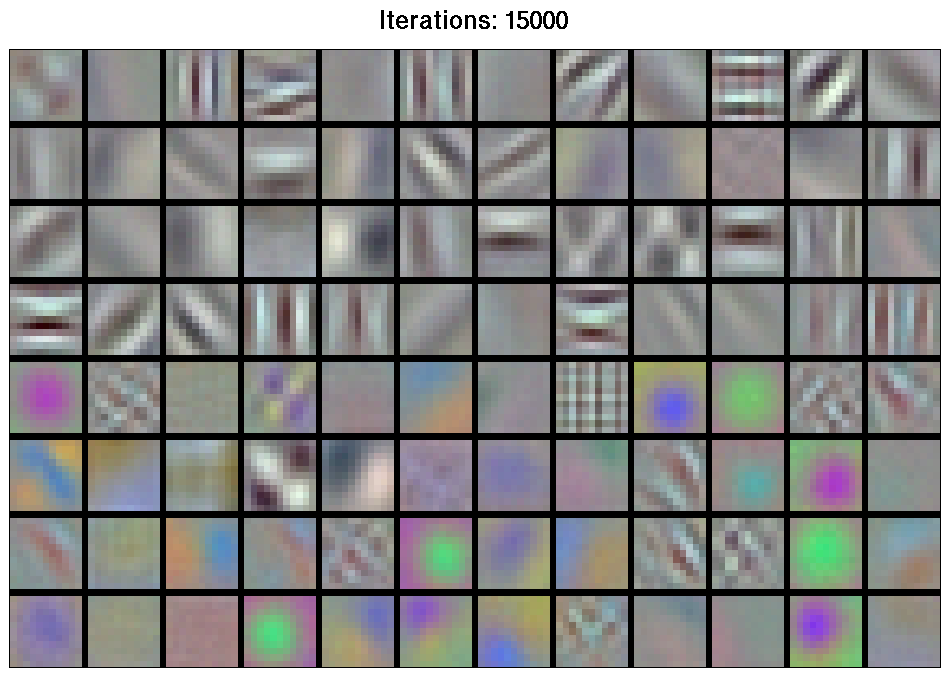
\includegraphics[scale=0.10]{images/l1_filters_iter15000.png}} \hspace{2mm}
\subfloat[305K Iterations]{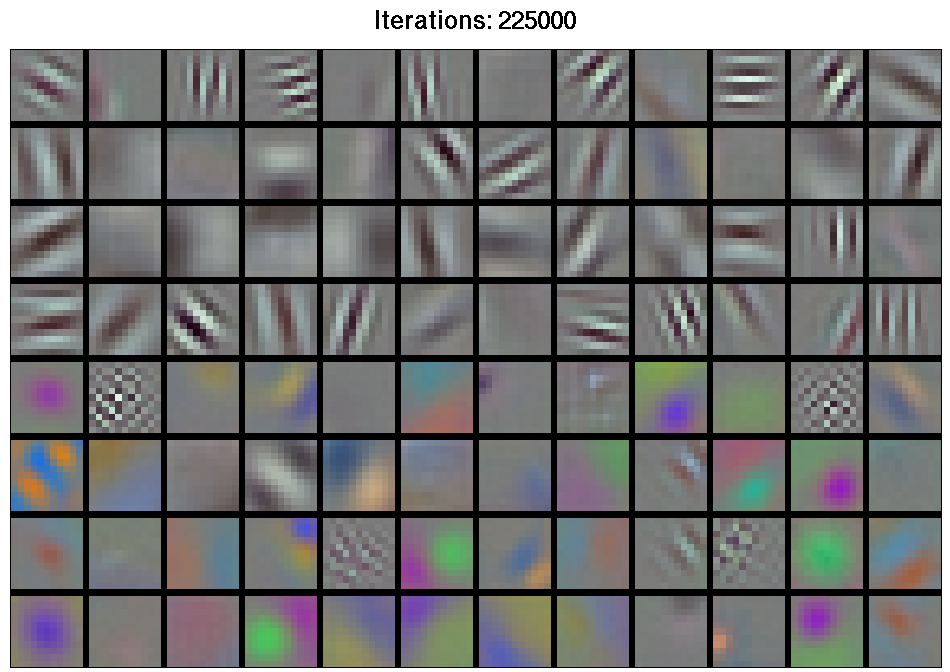
\includegraphics[scale=0.10]{images/l1_filters_iter225000.png}}
\caption{(a),(b),(c) show conv-1 filters after 5K, 15K and 305K iterations of training respectively. Notice, that just after 15K iterations these filters closely resemble their final state.}
\begin{comment} Note: I have labeled 305K as 225K - I cannot get the same shape as of the 5K, 15K for 305K. The filters look very similar and visually indistiguishable from 305K. If I have time later, I will make them all uniform.
\end{comment}
\label{fig:conv1}
\end{figure}

Performance on PASCAL-CLS as a function of pre-training time is reported in table \ref{table:det-traj-classify}. Notice, that more pre-training leads to better performance. It is noteworthy that by 15K and 50K iterations all layers are close to 80\% and  90\% of there final performance (recall, 1 epoch $\sim$ 5K iterations) respectively. This indicates that training required for generalization takes place quite quickly. Figure \ref{fig:conv1} shows conv-1 filters after 5K, 15K and 305K iterations and reinforces this observation. Further, notice that conv-1 trains first and the higher the layer is -  the more time it takes to converge. This suggests that a CNN by itself trains in layer by layer fashion.   

Table \ref{table:det-trajectory} reports results on SUN-CLS and PASCAL-DET and indicates that more pre-training prior to fine-tuning also leads to better performance.  


%The above analysis reinforces our belief that indeed majority of training required for generalization happens quite quickly as compared to the full training time of the network. This observation suggest that there may exist clever ways which can help us speed up the training.

